\documentclass[tikz,border=2pt]{standalone}
\usepackage{tikz}
\usetikzlibrary{calc}
\definecolor{olivegreen}{rgb}{0,0.6,0}
\begin{document}
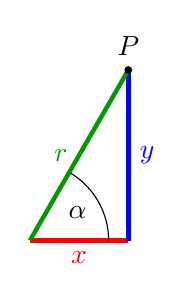
\begin{tikzpicture}
  \draw[ultra thick,red] (0,0) -- (60:2.5cm |- 0,0) node[midway,below] {$x$};
  \draw (1,0) arc (0:60:1) node at ($(60/2:0.7)$) {$\alpha$};
  \draw[ultra thick,blue] (60:2.5cm) -- (60:2.5cm |- 0,0) node[midway,right] {$y$};
  \draw[ultra thick,olivegreen,rotate=60] (0,0) -- node[midway,left] {$r$} (2.5,0) coordinate (B);
  \draw[xshift=-1cm] (B) node[circle,fill,inner sep=1pt,label=above:$P$] (e) {};
\end{tikzpicture}
\end{document}
